\subsection{Wyniki dyskretyzacji}
Dla każdego zbioru danych zostały przedstawione rozkłady wartości atrybutów. Pierwszy zawsze
przedstawia dane nieprzetworzone, natomiast 3 kolejne -- dane po zastosowaniu wyżej wymienionych
metod dyskretyzacji.

W celu wyznaczenia parametru określającego liczbę kubełków w metodach \textit{equal-width}
oraz \textit{equal-frequency}, została zastosowana reguła
\textbf{Freedmana-Diaconisa}:
    $$ nb\_bins = \frac{2 * IQR(data)}{\#data^{1/3}}$$

Stąd otrzymano następujące wartości (algorytm CAIM samodzielnie wyznacza liczbę kubełków):
\begin{itemize}
    \item{Zbiór \textbf{Diabetes} -- 14 kubełków (CAIM -- 2 kubełki),}
    \item{Zbiór \textbf{Glass} -- 2 kubełków (CAIM -- 6 kubełki),}
    \item{Zbiór \textbf{Wine} -- 4 kubełków (CAIM -- 3 kubełki),}
\end{itemize}


\subsubsection{Zbiór danych - "Diabetes"}
    Zbiór składa się z 8 atrybutów: zarówno dyskretnych (np. wiek), jak i ciągłych.
    Rozkład wartości 4 z nich przypomina rozkład normalny (glukoza, ciśnienie, BMI
    oraz pedigree). Gaussowski naiwny klasyfikator powinien sobie w miarę dobrze poradzić
    z tymi danymi.

    \begin{figure}[H]
        \center
        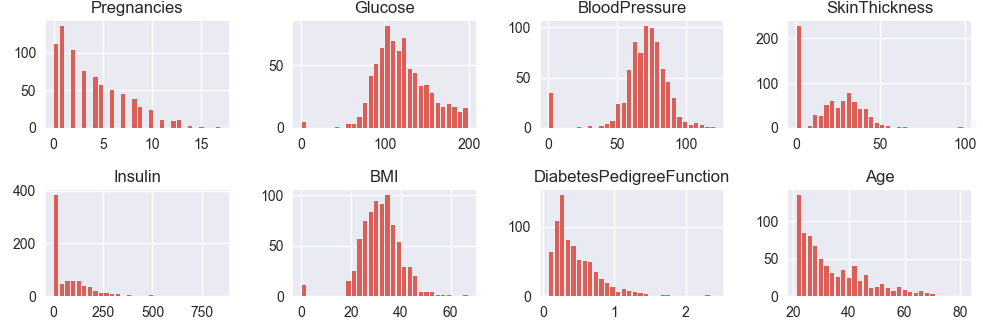
\includegraphics[width=0.7\textwidth]{img/discretization/non_discretized_diabetes.png}
        \caption{Rozkłady atrybutów zbioru "Diabetes" -- brak dyskretyzacji.}
    \end{figure}

    Ze względu na dość dużą liczbę wyznaczonych kubełków rozkłady z dyskretyzacją
    \textbf{equal-width} mocno przypominają rozkłady danych nieprzetworzonych (mała
    utrata informacji).

    \begin{figure}[H]
        \center
        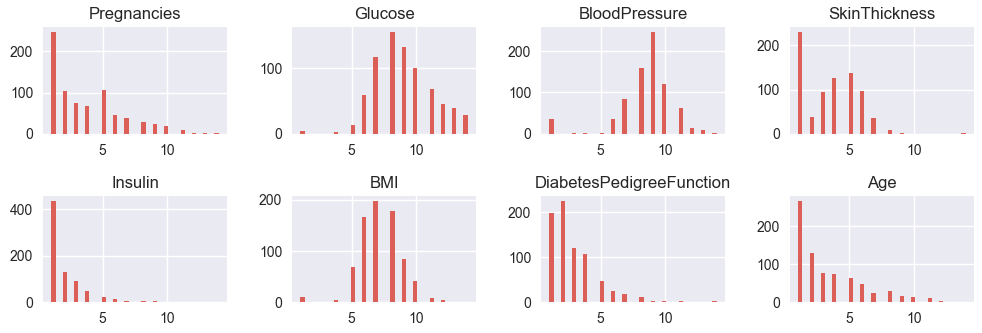
\includegraphics[width=0.7\textwidth]{img/discretization/ew_diabetes.png}
        \caption{Rozkłady atrybutów zbioru "Diabetes" -- dyskretyzacja "equal-width".}
    \end{figure}

    W przypadku metody \textbf{equal-frequency} widać, że nie wszystkie kubełki są
    idealnie równoliczne, jednak większość zachowuje się w sposób oczekiwany (wyjątek: liczba ciąż).

    \begin{figure}[H]
        \center
        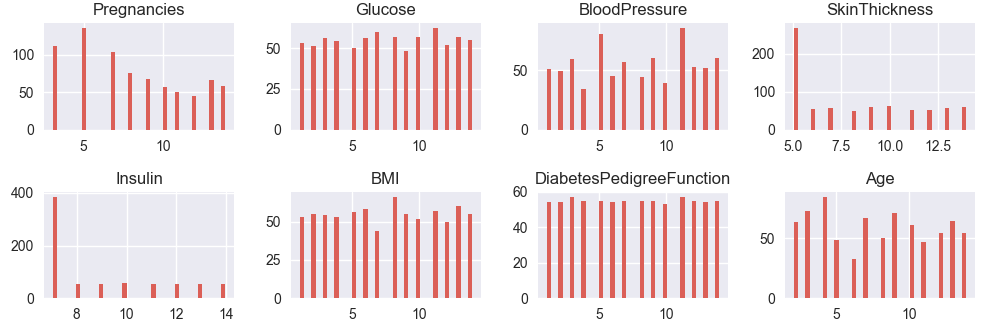
\includegraphics[width=0.7\textwidth]{img/discretization/ef_diabetes.png}
        \caption{Rozkłady atrybutów zbioru "Diabetes" -- dyskretyzacja "equal-frequency".}
    \end{figure}

    Metoda CAIM dobierając tylko 2 kubełki utraciła sporo informacji, jednak nie oznacza
    to, że będzie otrzymywała gorsze wyniki. Zarówno dla ciśnienia krwi, jak i pedigree
    można zauważyć, że rozkład jest bardzo niepropocjonalny i większość wartości atrybutów
    znalazła się w pierwszym kubełku.

    \begin{figure}[H]
        \center
        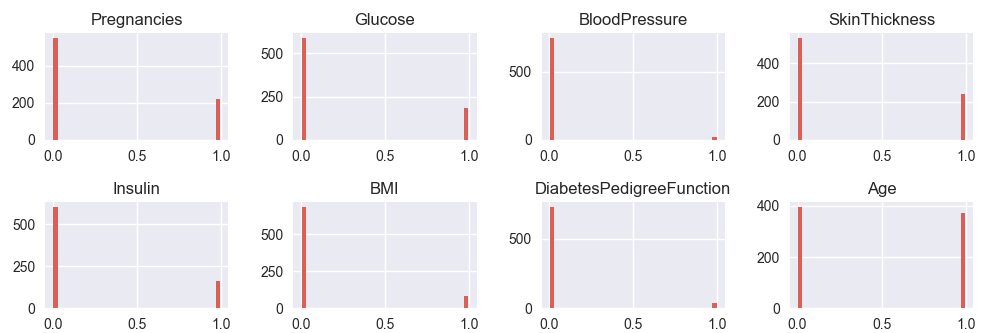
\includegraphics[width=0.7\textwidth]{img/discretization/caim_diabetes.png}
        \caption{Rozkłady atrybutów zbioru "Diabetes" -- dyskretyzacja "CAIM".}
    \end{figure}

\pagebreak
\subsubsection{Zbiór danych - "Glass"}
    Zbiór ten zawiera 9 atrybutów określających skład chemiczny szkła (pierwiastki).
    Niemalże wszystkie, za wyjątkiem K (potasu), Ba (baru) oraz Fe (żelaza), posiadają
    rozkłady wartości zbliżone do rozkładu normalnego. Gaussowski klasyfikator powinien
    tutaj sprawdzić się najlepiej.

    \begin{figure}[H]
        \center
        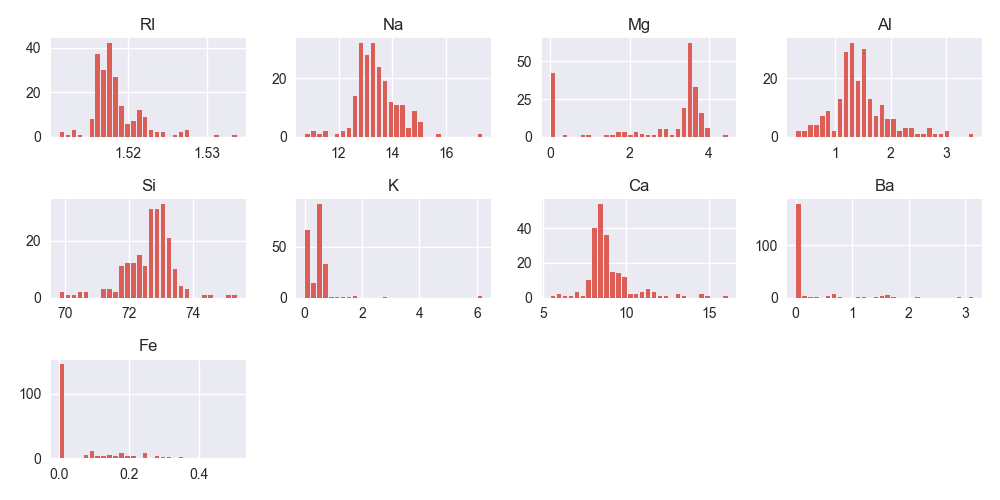
\includegraphics[width=0.7\textwidth]{img/discretization/non_discretized_glass.png}
        \caption{Rozkłady atrybutów zbioru "Glass" -- brak dyskretyzacji.}
    \end{figure}

    Podobnie jak w przypadku CAIM w poprzednim zbiorze danych, tak tutaj również nastąpiła
    spora utrata informacji, po przyjęciu 2 kubełków. Dla niektórych atrybutów dyspropocja
    w zapełnieniu kubełków jest skrajna (K, Ba, Fe) i są to te same, których rozkład nie
    przypominał rozkładu normalnego.

    \begin{figure}[H]
        \center
        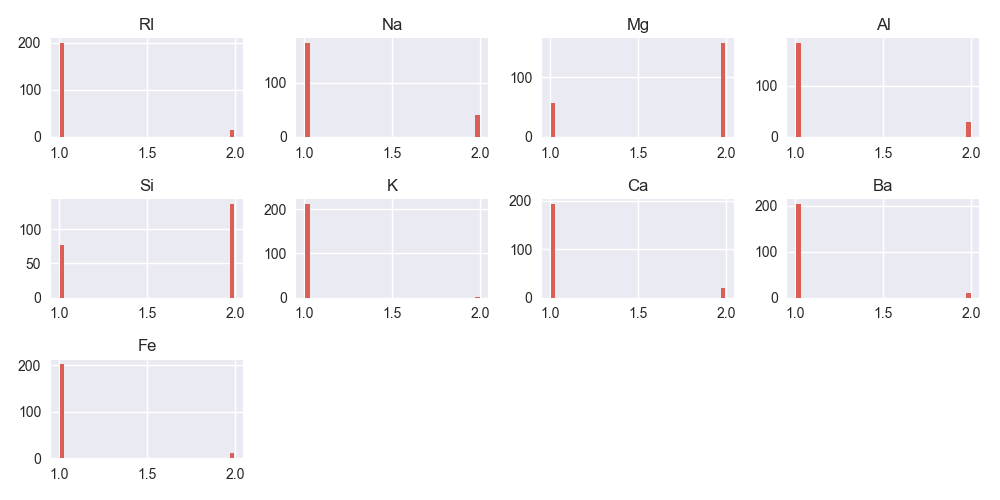
\includegraphics[width=0.7\textwidth]{img/discretization/ew_glass.png}
        \caption{Rozkłady atrybutów zbioru "Glass" -- dyskretyzacja "equal-width".}
    \end{figure}

    \pagebreak
    Metoda \textbf{equal-frequency} prawie idealnie rozłożyła wartości do dostępnych
    kubełków, jednak dla dwóch atrybutów (Ba, Fe) pojawiły się anomalie i wartości
    trafiły tylko do jednego kubełka.

    \begin{figure}[H]
        \center
        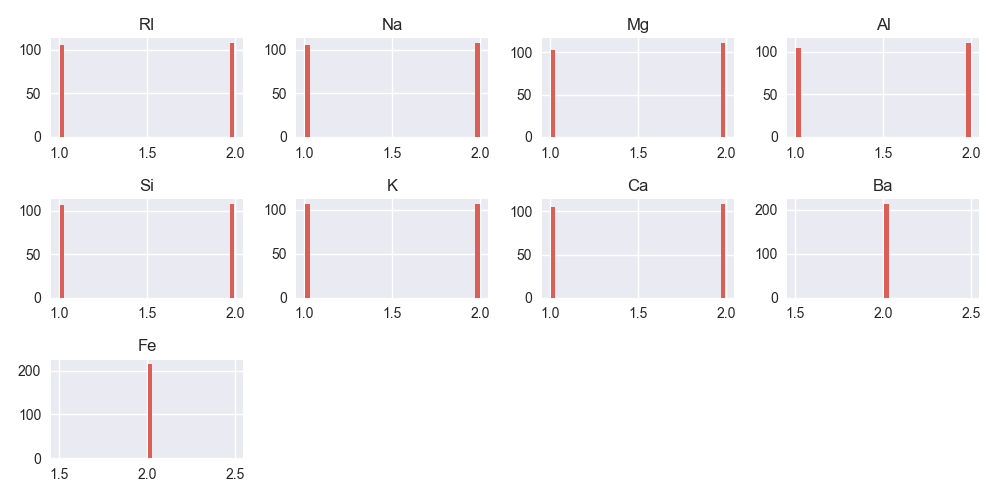
\includegraphics[width=0.7\textwidth]{img/discretization/ef_glass.png}
        \caption{Rozkłady atrybutów zbioru "Glass" -- dyskretyzacja "equal-frequency".}
    \end{figure}

    Algorytm CAIM poradził sobie tutaj znacznie lepiej. Dzieląc przedział wartości
    atrybutów na 6 kubełków, udało się zachować charakterystyki danych atrybutów (rozkładów atrybutów).

    \begin{figure}[H]
        \center
        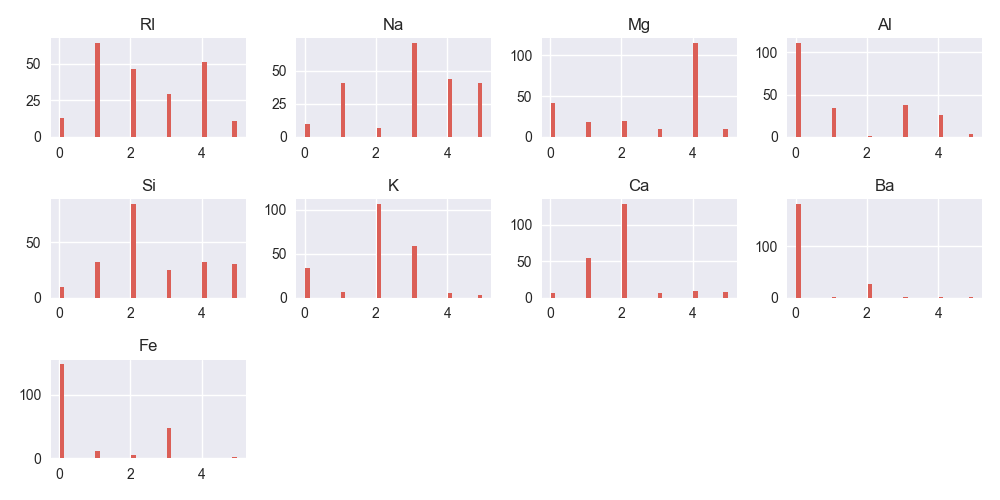
\includegraphics[width=0.7\textwidth]{img/discretization/caim_glass.png}
        \caption{Rozkłady atrybutów zbioru "Glass" -- dyskretyzacja "CAIM".}
    \end{figure}
    
\pagebreak
\subsubsection{Zbiór danych - "Wine"}
    Zbiór ten składa się 13 atrybutów, które określają pewne parametry
    charakterystyczne dla win. Tylko kilka spośród nich posiada rozkład normalny,
    zatem ten zestaw idealnie nadaje się do dyskretyzacji i użycia wielomianowego
    klasyfikatora. Rozkłady większości atrybutów wydają się być zaszumione lub podążać
    za kilkoma rozkładami normalnymi.

    \begin{figure}[H]
        \center
        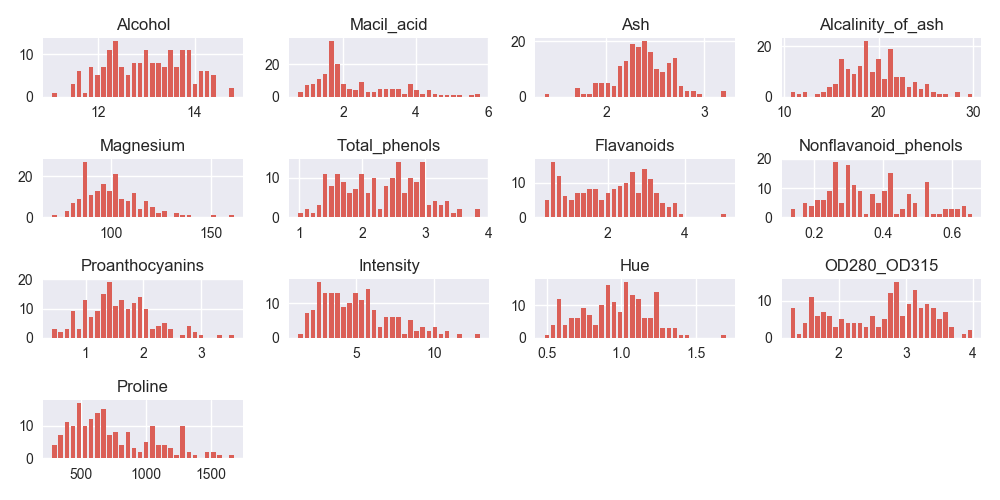
\includegraphics[width=0.75\textwidth]{img/discretization/non_discretized_wine.png}
        \caption{Rozkłady atrybutów zbioru "Wine" -- brak dyskretyzacji.}
    \end{figure}

    Dyskretyzacja \textbf{equal-width} przy parametrze liczby kubełków równej 4, bardzo
    dobrze odzwierciedlają nieprzetworzone rozkłady, jednocześnie eliminując "szumy".
    Zatem ta metoda dobrze zgeneralizowała i wyodrębniła istotę poszczególnych rozkładów.

    \begin{figure}[H]
        \center
        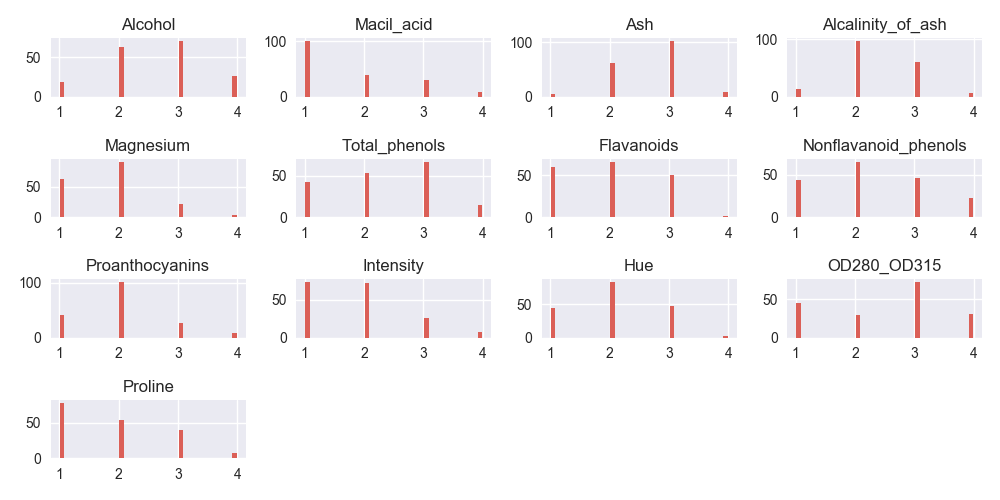
\includegraphics[width=0.75\textwidth]{img/discretization/ew_wine.png}
        \caption{Rozkłady atrybutów zbioru "Wine" -- dyskretyzacja "equal-width".}
    \end{figure}

    \pagebreak
    Metoda \textbf{equal-frequency} w tym wypadku dla każdego atrybutu równomiernie
    rozłożyła wartości. Nie było tak dużych rozbieżności jak w przypadku poprzednich
    zbiorów danych.

    \begin{figure}[H]
        \center
        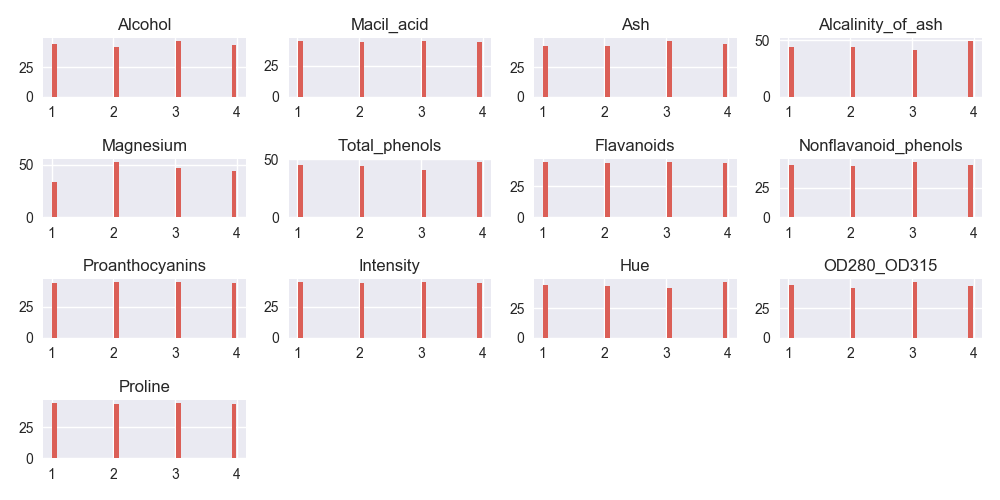
\includegraphics[width=0.75\textwidth]{img/discretization/ef_wine.png}
        \caption{Rozkłady atrybutów zbioru "Wine" -- dyskretyzacja "equal-frequency".}
    \end{figure}

    Dyskretyzacja \textbf{CAIM} używa w tym zbiorze danych tylko 3 kubełków. W części
    przypadków odbiegają od początkowych, nieprzetworzonych rozkładów -- np. atrybut
    \textit{Proline} więcej wartości ma przy mniejszych wartościach (skupione głównie
    wokół 500), natomiast CAIM dla pierwszego kubełka posiada najmniej wartości.

    \begin{figure}[H]
        \center
        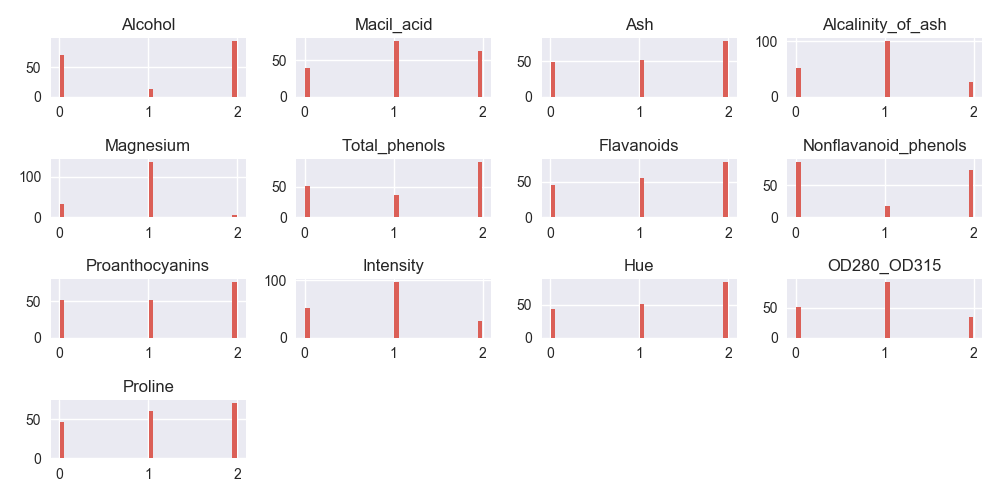
\includegraphics[width=0.75\textwidth]{img/discretization/caim_wine.png}
        \caption{Rozkłady atrybutów zbioru "Wine" -- dyskretyzacja "CAIM".}
    \end{figure}
